% Springer proceedings manuscript (official LaTeX2e Proceedings Template,
% llncs.cls v2.25, 2026-09-03; bibliography style splncs04).
% Main file: compile with pdfLaTeX + BibTeX (Overleaf default).
% Author metadata lives in metadata.tex; each section in sections/; tables in
% tables/; figures in figures/; references in references.bib.
\documentclass[runningheads]{llncs}

\usepackage[T1]{fontenc}
\usepackage{newtxtext}
\usepackage[varvw]{newtxmath}
\usepackage{graphicx}
\usepackage{amsmath}
\usepackage{booktabs}
\usepackage{tikz}
\usetikzlibrary{arrows.meta,positioning}
\usepackage{xcolor}
\usepackage{url}
\usepackage[hidelinks]{hyperref}
% Springer eBook style for URLs (from the template):
\renewcommand\UrlFont{\color{blue}\rmfamily}
\urlstyle{rm}

\begin{document}

% =====================================================================
% AUTHOR METADATA -- edit ONLY this file for title and author block.
% Author block follows the author's own paper "Noise-Robust Quantum Machine
% Learning for Building Energy Performance" (name, department, school,
% university, city, country; no e-mail or ORCID line).
% =====================================================================

\title{Evaluating Record-Level Supervisory Analytics for Security Operations Centres:
Controlled Validation, Decision Integrity}

% Short title for the running head (used because the full title is long).
\titlerunning{Evaluating Record-Level Supervisory Analytics for SOCs}

\author{Pratham Kapoor}

% Running head: first names abbreviated.
\authorrunning{P. Kapoor}

\institute{Department of Information Technology\\
Mukesh Patel School of Technology Management \& Engineering\\
SVKM's NMIMS University, Mumbai, India}

\maketitle

\begin{abstract}
Supervisors of security operations centres must judge periodically whether monitored
organizations detect, investigate, escalate and close security work properly, yet
the usual instruments are self-assessed maturity models and manual record review.
We study whether the operational records an organization submits can instead be
analysed into findings that cite those records, ranked across organizations, decided
by a human supervisor, and bound to that decision cryptographically. We implement
this workflow as SAT-SA, with 16 deterministic rule-based workers, a
saturating risk fusion and a post-quantum signed, hash-chained receipt, and evaluate
it on frozen, hash-verified experiment bundles. On controlled data the mechanisms
behave as designed: every declared finding family was emitted, validation matched
its declared contract in all 245 perturbed conditions, all
13 tested mutations of the decided record were detected, and all
36 injected workflow interruptions recovered. Simple rules are, however,
competitive: fixed-threshold and median-deviation rules tied the fast-closure
detector, and a closure-speed heuristic nearly matched the ranking; stale and
contradictory records were accepted silently. On a public IT incident log, which is
not security-operations data, the risk score was not associated with service-level
misses (Spearman $\rho=\ensuremath{-}0.11$), while slowest median resolution was
($\rho=0.94$); a failure analysis attributes this to construct
mismatch and detector saturation. The evidence supports mechanism-level claims, not
effectiveness in real security operations, for which no human study or expert labels
exist.

\keywords{Security operations \and Supervisory analytics \and Incident management
\and Process conformance \and Human-in-the-loop decision support \and Post-quantum
signatures \and Negative results.}
\end{abstract}


\section{Introduction}
\label{sec:intro}

Security operations centres (SOCs) triage large alert volumes with limited analyst
capacity~\cite{vielberth2020soc,tariq2025alertfatigue}, and field studies document
recurring process problems: false-positive-dominated alarms, mismatched expectations
between analysts and management, and burnout~\cite{alahmadi2022falsepositives,kokulu2019soc,sundaramurthy2015burnout}.
When an external body supervises many SOCs---for example a national authority for
critical infrastructure---it must judge periodically whether each monitored
organization actually investigated, escalated and closed its work properly. The
instruments available are mostly maturity self-assessments such as
SOC-CMM~\cite{vanos2016soccmm} and CTI-SOC2M2~\cite{schlette2021ctisoc2m2}, metric
catalogues~\cite{forsberg2023metrics,agyepong2023analyst}, and manual examination of
records. Self-assessment reports capability, not conduct; manual examination does not
scale across many organizations and periods.

Record-based assessment of incident handling is not new. Palma et al.\ assess the
compliance of an incident-management process with a reference model derived from
ITIL and ISO/IEC~27035 by aligning its event log with that model and prioritizing
the deviations for an auditor~\cite{palma2024compliance,palma2024benchimp}, and
support the assessor with visual analytics~\cite{palma2024eurova,palma2025impavid}.
SOC performance has also been measured empirically by injecting synthetic attacks
into an operational SOC~\cite{rosso2020saibersoc}. What remains open for the
supervisory setting is narrower: an analysis of the heterogeneous records a monitored
SOC submits (alerts, cases, investigation steps, escalations, dispositions, assets)
that yields findings citing those records, ranks organizations against each other,
keeps a human supervisor as the decision authority, and makes the decided state
verifiable afterwards---together with an honest account of how such an analysis
behaves on controlled and on independent data.

This paper studies that question with an implemented system, SAT-SA (developed for
the Smart India Hackathon problem SIH26157), and a frozen evaluation. Its emphasis is
the evidence rather than the architecture: every number is taken from a hash-verified
experiment bundle, and negative findings are reported with the same prominence as
positive ones.

\paragraph{Contributions.} We separate contribution types and state their strength.
\begin{itemize}
\item \emph{Application framing (low-confidence candidate).} Supervisor-side,
record-level analytics over SOC evidence submissions, with findings that cite
records, cross-organization peer comparison, entity ranking and a bound human
decision. Each ingredient has prior art (Section~\ref{sec:related}); the combination
is offered without a novelty claim.
\item \emph{Empirical findings.} Controlled evaluations of detection against declared
labels and simple baselines, one-worker ablation, imperfect-evidence robustness,
peer-cohort sensitivity, orchestration cost and recovery, and an external negative
result on a public IT incident log with a construct-level failure analysis.
\item \emph{Engineering.} A tenant-aware submission, analysis and review workflow with
a durable queue and a checkpointed human-review interrupt.
\item \emph{Security capability (integration).} Binding of the supervisory decision to
the analysed state with standard primitives (SHA3-256, ML-DSA-65, a hash-chained
ledger), evaluated with a mutation matrix.
\item \emph{Reproducibility practice.} Write-once experiment bundles, an evidence
freeze and a data layer that generates every reported number.
\end{itemize}
We make no claim of algorithmic novelty, superiority over existing systems, or
effectiveness in real SOCs.

The remainder of the paper reviews related work (Section~\ref{sec:related}), formalizes
the problem and the implemented analysis (Sections~\ref{sec:formulation}
and~\ref{sec:system}), describes the experimental methodology
(Section~\ref{sec:method}), reports controlled results (Section~\ref{sec:results}) and
the external evaluation (Section~\ref{sec:external}), and discusses implications,
threats to validity and reproducibility (Sections~\ref{sec:discussion}--\ref{sec:repro}).

\section{Related Work and Research Gap}
\label{sec:related}

\paragraph{Literature search and positioning.} We positioned the work with a
structured search, not a systematic review. Twenty queries on SOC assessment, alert prioritization, security
process mining, peer analytics, supervisory technology and tamper-evident records
were run on OpenAlex and Crossref in September 2026 for publications from 2005
onwards (656 unique records, screened in a single pass; 106 abstracts
read; 51 included and joined with 26 sources of an earlier focused review), followed
by an update search for closest prior art and counterevidence. arXiv throttled the
automated queries and records beyond rank 25 per query were not screened, so absence
from this review is not evidence of absence. Queries, counts and decisions are in
the supplementary material.

\paragraph{SOC assessment and measurement.} Maturity models score capability through
self- or expert assessment~\cite{vanos2016soccmm,schlette2021ctisoc2m2}; metric
work defines and weights indicators of analyst or technical
performance~\cite{agyepong2019review,agyepong2023analyst,forsberg2023metrics}.
A case study in one academic SOC found that analysts who scored well on key
performance indicators did not necessarily further the SOC's goals~\cite{morin2025mismatched},
a caution for any metric-based supervision. SAIBERSOC measures an operational SOC
empirically by injecting synthetic attacks and observing outputs such as detection
accuracy and time to investigation, in an experiment with 124 students acting as
analysts~\cite{rosso2020saibersoc}. These approaches assess capability or test a SOC
actively; none analyses the records a SOC submits to an external supervisor.

\paragraph{Record-based assessment of incident handling (closest prior art).}
Palma et al.\ built a system that assesses an organization's incident-management
process for compliance with a reference process derived from ITIL and ISO/IEC~27035:
it aligns the event log with the model, classifies deviations with a taxonomy,
prioritizes them with a cost model and supports an auditor; it was validated on a
benchmark and demonstrated on a public real incident-management log~\cite{palma2024compliance}.
A companion benchmark compares such assessment models~\cite{palma2024benchimp}, and
two visual-analytics tools support the human assessor~\cite{palma2024eurova,palma2025impavid}.
The public log used in that line of work is the ServiceNow incident log (141,712 events
over 24,918 incidents) released with~\cite{amaral2019completion} and published
as~\cite{amaral2018uci498}---the same log we use for our external evaluation, and one
on which SLA attainment has also been modelled directly~\cite{swain2022sla}. Automated,
record-based assessment of incident handling for an assessor therefore already exists
and has been demonstrated on our external data. Table~\ref{tab:related} contrasts it
with SAT-SA.

\begin{table}[t]
\caption{Closest prior work compared with SAT-SA, as described in the cited sources
(``--'' not addressed; ``n/d'' not determinable from the source).}
\label{tab:related}
\centering
\scriptsize
\setlength{\tabcolsep}{2.5pt}
\begin{tabular}{@{}p{2.1cm}p{2.1cm}p{2.1cm}p{1.7cm}p{1.5cm}p{1.5cm}@{}}
\toprule
Work & Evidence & Analysis & Across organizations & Human role & Decision binding \\
\midrule
Maturity models \cite{vanos2016soccmm,schlette2021ctisoc2m2} & self / expert assessment & maturity scoring & comparable scores & assessor & -- \\
SAIBERSOC \cite{rosso2020saibersoc} & outputs of an operational SOC & synthetic attack injection & SOC configurations & analysts & -- \\
Palma et al.\ \cite{palma2024compliance,palma2025impavid} & incident-management event log & alignment, deviation cost model & n/d & auditor, assessor & -- \\
DomainPrio \cite{chiba2022domainprio} & one SOC's investigations & population analysis, regression & -- & analysts & -- \\
SAT-SA (this work) & six categories of submitted SOC records & rule-based workers, saturating fusion & peer cohorts, ranking & supervisor decides & signed receipt, ledger \\
\bottomrule
\end{tabular}
\end{table}


\paragraph{Alert and incident prioritization.} A large literature ranks alerts or
incidents for analysts~\cite{jalalvand2024prioritisation,tariq2025alertfatigue}:
resource-aware selection of alerts to investigate~\cite{shah2019alertselection},
provenance-based triage~\cite{hassan2019nodoze}, guided response learned from
customer triage labels~\cite{freitas2024guide}, learning to defer to
analysts~\cite{jalalvand2025l2d}, and, recently, LLM agents embedded in SOC
triage~\cite{banstola2026agentic}. DomainPrio analyses the population of a SOC's
investigations rather than single alerts~\cite{chiba2022domainprio}. SAT-SA differs in
unit and user---it ranks monitored organizations for a supervisor from findings about
how work was handled---and is not compared with these systems.

\paragraph{Process conformance and peer comparison.} Conformance checking relates
recorded behaviour to a model and exposes skipped or out-of-order
activities~\cite{rozinat2008conformance,carmona2018conformance,vanderaalst2016pm},
and has been applied to security audit trails~\cite{vanderaalst2005security} and to
IT incident management against ITIL~\cite{ferreira2008itil}. SAT-SA's execution-gap
and negative-space rules are rule-encoded conformance checks, not a new technique.
Peer group analysis flags entities that diverge from similar
entities~\cite{weston2008pga,bolton2002fraud}; SAT-SA uses median and median absolute
deviation (MAD)~\cite{leys2013mad} over a declared cohort.

\paragraph{Supervision and human oversight.} Financial supervisors use technology to
analyse submitted data (``suptech'') while keeping human judgement
central~\cite{broeders2018suptech}. Automation bias is a documented risk of decision
support~\cite{parasuraman2010automation} and has been reviewed for SOCs
specifically~\cite{tilbury2024automationbias}; we did not study it.

\paragraph{Integrity of records.} Tamper-evident logs detect alteration of recorded
history~\cite{schneier1999logs,crosby2009logging}; practical systems protect audit logs
with trusted execution~\cite{paccagnella2020custos} or ratcheting~\cite{guardiola2022sealfs},
and post-quantum primitives have been applied to forensic logging~\cite{fugkeaw2026pqabl}.
SAT-SA proposes no logging scheme or cryptography; it composes
SHA3-256~\cite{nist2015fips202} and ML-DSA-65~\cite{nist2024fips204} to bind one
canonical supervisory record to the authorized decision.

\paragraph{Gap.} Record-based incident assessment, supervisory analysis of submitted
data, peer comparison and tamper-evident records each exist. Within the databases,
queries, screening procedure and time period described above, we did not identify a
study that combines them for supervision of many SOCs from their evidence submissions---with
record-cited findings, cross-organization ranking and a cryptographically bound human
decision---and evaluates the combination against simple baselines and on independent
data. This is a search-bounded observation about a combination of established parts,
not a claim that no such study exists.

\section{Problem Formulation}
\label{sec:formulation}

We formalize the workflow as it is implemented; no step below is learned from data.

\paragraph{Submissions.} For a monitored organization (entity) $e$ and assessment
period $t$, a \emph{submission} $S_{e,t}$ is a versioned set of records partitioned
into six evidence categories (alerts, cases, investigation steps, escalations,
dispositions, assets). Each record $r$ carries its source provenance (artifact digest
and record locator). Validation is a total function
$V(S_{e,t})\in\{\mathit{accept},\mathit{reject}\}$ that parses every record, resolves
references (e.g.\ a step must reference an existing case) and enforces chronology; it
is all-or-nothing, so a single invalid record rejects the version.

\paragraph{Findings.} Each analytical worker $w_j$, $j=1,\dots,16$, maps
an accepted submission (and, for peer analysis, a declared cohort) to findings
\begin{equation}
f=(\rho_f,\ \mathit{subject}_f,\ E_f,\ s_f,\ \theta_f,\ c_f),
\end{equation}
with rule $\rho_f$, subject, evidence references $E_f\subseteq S_{e,t}$, statistic $s_f$,
threshold $\theta_f$ and confidence $c_f\in[0,1]$. A finding is a \emph{signal} only if
$E_f\neq\emptyset$; findings without evidence references are withheld. Let $F_e$ be the
signal findings of the entity's run.

\paragraph{Rule families.} Most execution-gap rules are \emph{existence rules}: they
fire when at least one qualifying record exists, e.g.\ a critical alert closed faster
than a severity-specific limit. Peer deviation compares an entity metric $x_e$ with the
median $\tilde m$ and median absolute deviation $\mathrm{MAD}$ of a declared cohort
$C$ (after symmetric 10\% trimming when $|C|\ge 4$) and fires when
\begin{equation}
|C|\ge 3 \quad\text{and}\quad |x_e-\tilde m| \ge 2\,\mathrm{MAD}(C);
\label{eq:peer}
\end{equation}
within-entity anomalies use the same statistic with factor $3$ over the entity's own
values. MAD is unscaled.

\paragraph{Risk fusion.} A fixed map $\delta$ assigns each rule to one of
$7$ dimensions $d$ with weights $w_d$ (execution gap
25, peer deviation 20, detection gap
15, negative space 15, anomaly
15, investigation quality 5,
escalation discipline 5; sum 100). With
$C_d=\sum_{f\in F_e,\ \delta(\rho_f)=d} c_f$,
\begin{equation}
R_d = w_d\,\frac{C_d}{1+C_d},\qquad R_e=\min\Bigl(100,\ \sum_d R_d\Bigr).
\label{eq:risk}
\end{equation}
Each dimension saturates at its weight. Two properties matter later: $R_e$ is a
heuristic score, not a probability or a severity; and it depends on summed confidences,
not on how \emph{prevalent} a problem is within the submission. Findings from different
families naming the same subject are reported as corroborating clusters that do not
change $R_e$.

\paragraph{Prioritization.} Entities are ordered by the priority score
\begin{equation}
P_e = R_e + 10\,\kappa_e + 5\,\tau_e + 2\,h_e,
\label{eq:priority}
\end{equation}
where $\kappa_e\in\{0,\tfrac14,\tfrac35,1\}$ encodes the confidence bucket of the entity's
findings, $\tau_e\in[0,1]$ decays linearly with run age over 30 days, and $h_e$ counts
high-severity signals. The coefficients are fixed defaults, not fitted.

\paragraph{Decision and binding.} A supervisor (or organization administrator)
records a decision $D_e$ on the reviewed state. Finalization builds a canonical
document $\mathit{doc}_e$ (decision, findings, observations, risk, recommendations,
submission records and their provenance), computes $h_e=\mathrm{SHA3\text{-}256}(\mathit{doc}_e)$,
signs $h_e$ with ML-DSA-65, stores a receipt, and appends a ledger entry
$\ell_i$ whose hash is $\mathrm{SHA3\text{-}256}$ of its canonical body including the
predecessor hash $\ell_{i-1}$. Verification rebuilds $\mathit{doc}_e$ from the live
records and checks the digest, the decision binding, the signature and the chain.

\paragraph{Questions.} Given this pipeline, we ask whether the declared mechanisms
behave as specified under controlled conditions, how they compare with simple
baselines, how they respond to imperfect evidence and cohort choice, what orchestration
and integrity cost, and whether $R_e$ tracks an independent outcome on real data
(Section~\ref{sec:method}).

\section{System Architecture and Analytical Methodology}
\label{sec:system}

Figure~\ref{fig:architecture} shows the workflow as implemented. An analyst of the
monitored organization uploads one file per evidence category through an HTTP API;
validation stores per-record provenance; a separate worker process claims queued
runs under a lease and executes the analysis; a supervisor reviews and decides; and
the decision is finalized and bound.

\begin{figure}[!htbp]
\centering
% Figure 1 -- SAT-SA workflow (native TikZ; edit labels directly).
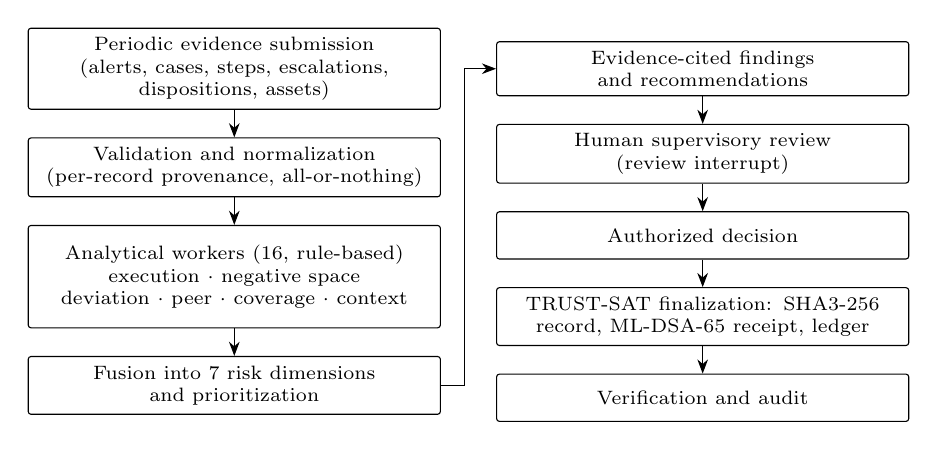
\begin{tikzpicture}[node distance=3.5mm and 6mm, every node/.style={font=\scriptsize},
  box/.style={draw, rounded corners=1pt, align=center, text width=50mm, minimum height=6mm},
  arr/.style={-{Stealth[length=1.8mm]}}]
\node[box] (sub) {Periodic evidence submission\\(alerts, cases, steps, escalations,\\dispositions, assets)};
\node[box, below=of sub] (val) {Validation and normalization\\(per-record provenance, all-or-nothing)};
\node[box, below=of val, minimum height=13mm] (ana) {Analytical workers (16, rule-based)\\execution $\cdot$ negative space\\deviation $\cdot$ peer $\cdot$ coverage $\cdot$ context};
\node[box, below=of ana] (risk) {Fusion into 7 risk dimensions\\and prioritization};
\node[box, right=7mm of sub] (find) {Evidence-cited findings\\and recommendations};
\node[box, below=of find] (rev) {Human supervisory review\\(review interrupt)};
\node[box, below=of rev] (dec) {Authorized decision};
\node[box, below=of dec] (trust) {TRUST-SAT finalization: SHA3-256\\record, ML-DSA-65 receipt, ledger};
\node[box, below=of trust] (ver) {Verification and audit};
\draw[arr] (sub) -- (val); \draw[arr] (val) -- (ana); \draw[arr] (ana) -- (risk);
\draw[arr] (risk.east) -| ++(3mm,0) |- (find.west);
\draw[arr] (find) -- (rev); \draw[arr] (rev) -- (dec); \draw[arr] (dec) -- (trust); \draw[arr] (trust) -- (ver);
\end{tikzpicture}

\caption{SAT-SA supervisory workflow along the evaluated path. The analytical-worker
stage is the evaluated subset of the registered agents (Table~\ref{tab:architecture}).
All analytics are deterministic and rule-based; orchestration (direct worker or
LangGraph) sequences the stages and pauses for the human decision.}
\label{fig:architecture}
\end{figure}

\subsection{Architecture layers}
The implementation registers 32 components that it calls
\emph{agents} (Table~\ref{tab:architecture}): 23 supervisory agents
and 9 MLOps agents retained from the platform SAT-SA was built on.
An agent here is a registered specification (purpose, inputs, outputs, evidence types)
that maps to deterministic code; none is a language-model or autonomous agent. Eleven
supervisory agents cover the analysis families and group the 16 default
analytical workers evaluated in this paper; the other twelve cover the pipeline around
them, from ingestion and normalization through correlation, risk scoring,
prioritization and recommendation to review, trust and provenance, reporting and
validation. The reported experiments exercise the analytical workers and the
pipeline from ingestion to trust; evidence assembly, meta-audit, report generation,
the calibration-oriented validation agent and the retained MLOps agents are not
evaluated. The count of 16 therefore refers to the analytical workers
only, not to the whole architecture.

\begin{table}[!htbp]
\caption{SAT-SA architecture inventory as implemented. ``Agent'' is the
implementation's name for a registered component; each maps to deterministic code, and
none is a language-model or autonomous agent. Only the rows marked ``yes'' are exercised
by the reported experiments.}
\label{tab:architecture}
\centering
\small
\setlength{\tabcolsep}{3pt}
\begin{tabular}{@{}L{3.5cm}L{1.0cm}L{5.1cm}L{1.8cm}@{}}
\toprule
Layer & Count & Members & Evaluated \\
\midrule
Registered agents (agent registry) & 32 & 23 supervisory agents and 9 retained MLOps agents & in part \\
\quad Supervisory analytical agents & 11 & one agent per analysis family; they group the 16 default analytical workers (the execution-gap agent groups six detectors) & yes \\
\quad Supervisory pipeline agents & 12 & ingestion, normalization, correlation, risk scoring, prioritization, recommendation, review workflow, trust--provenance, evidence assembly, meta-audit, report generation, validation & ingestion to trust: yes; last four: no \\
\quad Retained MLOps agents & 9 & data, performance, security, quantum security, red team, training optimization, incident response, governance, optimization (inherited platform) & no \\
Default analytical workers & 16 & listed in Tables~\ref{tab:workers} and~\ref{tab:workers-b} & yes \\
Orchestration graph nodes & 5 & readiness, analysis, recommendations, human review, trust boundary (LangGraph mode) & yes \\
\bottomrule
\end{tabular}
\end{table}


\subsection{Analytical workers}
The 16 default analytical workers fall into five functional groups.
\emph{Execution and process rules} (fast closure, acknowledgement without
investigation, critical alert without escalation, repeated shallow investigation,
recurrence without remediation, potential metric gaming) check individual records and
short record chains against expected handling. \emph{Negative-space analysis} detects
the absence of expected work: cases without investigation steps, missing escalations
or dispositions, critical assets without alerts; these are rule-encoded conformance
checks. \emph{Deviation analysis} comprises within-entity anomalies, drift and the peer
rule of Eq.~\eqref{eq:peer}. \emph{Coverage and completeness} (coverage gap, evidence
completeness) flag unmonitored assets and missing evidence categories, and
entity--asset resolution links records to the assets they concern. \emph{Context workers} (workflow reconstruction, case similarity,
cross-entity insights) reconstruct sequences and clusters; their signals also feed risk
dimensions. Tables~\ref{tab:workers} and~\ref{tab:workers-b} list all 16 workers with the
dimension each feeds and its confidence rule. Because a rule's dimension is assigned by
name prefix, the escalation-discipline and investigation-quality dimensions are fed only
by workflow reconstruction (and by keyword-matching drift or cross-entity rules), while
critical alerts without escalation count towards the execution gap. No worker uses a
language model or a learned model.

\begin{table}[!htbp]
\caption{Default analytical workers evaluated in the reported experiments (part 1 of
2; the analytical subset of the registered agents, Table~\ref{tab:architecture}): risk
dimension fed and confidence components, $c_f=\min(a_f,e_f[,p_f])$
(Eq.~\eqref{eq:confidence}). $q$ = qualifying records; $N$ = records of the relevant
category; $\delta$ = effect size clipped to $[0,1]$; $z$ = deviation in MADs. All
constants are fixed in code. Dimensions: EG execution gap, NS negative space, AN
anomaly, PD peer deviation, DG detection gap, IQ investigation quality, ED escalation
discipline; kw = assigned by rule-name keyword (default AN).}
\label{tab:workers}
\centering
\small
\setlength{\tabcolsep}{3pt}
\begin{tabular}{@{}L{2.7cm}L{0.9cm}L{4.4cm}L{3.5cm}@{}}
\toprule
Worker & Dim. & Analytical support $a_f$ & Evidence completeness $e_f$ (peer $p_f$) \\
\midrule
Fast closure & EG & $0.4+0.6\,\delta$, $\delta=1-\text{median}/\text{limit}$ & $q/N$ (alerts of that severity) \\
Ack.\ without investigation & EG & $0.5+0.4\,q/N$ & $q/N$ (alerts) \\
Critical without escalation & EG & $0.8$ & $q/N$ (alerts) \\
Repeated investigation & EG & $0.4+0.5\,\delta$ & $\min(1,N_{\text{steps}}/20)$ \\
Recurrence without remediation & EG & $0.7$ & $q/N$ (cases) \\
Potential metric gaming & EG & $0.4+0.4\,\delta$ & $\min(1,N/20)$ \\
Negative space & NS & $0.7$ steps; $0.6$ escalation, monitoring; $0.5$ disposition; $0.4$ low activity & $1$ if category submitted, else $0$ \\
Anomaly & AN & $0.4+0.5\min(1,z/3)$ & $1$ \\
Peer benchmark & PD & $0.4+0.1\min(1,|z|/3)$ & $1$; $p_f=\min(1,n_{\text{peers}}/10)$ \\
Drift & kw & $0.4+0.6\min(1,|\Delta_{\text{rel}}|)$ & $0.9/0.6/0.3$ (${\ge}3$/${\ge}1$/$0$ refs) \\
\bottomrule
\end{tabular}
\end{table}

\begin{table}[!htbp]
\caption{Default analytical workers evaluated in the reported experiments (part 2 of
2); abbreviations as in Table~\ref{tab:workers}.}
\label{tab:workers-b}
\centering
\small
\setlength{\tabcolsep}{3pt}
\begin{tabular}{@{}L{2.7cm}L{0.9cm}L{4.4cm}L{3.5cm}@{}}
\toprule
Worker & Dim. & Analytical support $a_f$ & Evidence completeness $e_f$ (peer $p_f$) \\
\midrule
Coverage gap & DG & $0.4+0.6\,g$ ($g$ unmonitored critical-asset share) & $0.9$ if alerts link assets, else $0.4$ \\
Cross-entity insights & kw & $0.4+0.6\min(1,\pi)$ ($\pi$ prevalence) & $0.9$ if ${\ge}3$ entities, else $0.6$; $p_f=\min(1,\pi)$ \\
Case similarity & AN & $0.5+0.5\,s$ ($s$ cluster share) & $0.7$ \\
Evidence completeness & AN & $0.4+0.6\,m$ ($m$ missing share) & $1-m$ \\
Workflow reconstruction & ED, IQ, AN & $0.85$ / $0.8$ / $0.6$ by rule & $1$ \\
Entity--asset resolution & AN & $0.6$ & $1$ \\
\bottomrule
\end{tabular}
\end{table}


\subsection{Fusion, prioritization and recommendations}
Signal findings are fused by Eq.~\eqref{eq:risk} into an entity risk decomposed by
dimension, so that a supervisor sees which findings produce which part of the score.
Entities are ordered by Eq.~\eqref{eq:priority}, and each finding family maps to a
recommended supervisory action.

\subsection{Human supervisory review}
Runs can require review. The system does not make the final supervisory decision; the
authorized human reviewer (a supervisor or an organization administrator) records the
decision, after which the worker resumes.

\subsection{Stateful orchestration}
The same stages run in two modes. In \emph{direct} mode the worker pauses the run after
analysis and recommendations. In \emph{graph} mode a LangGraph~\cite{langgraph2026docs}
graph with 5 nodes (readiness, analysis, recommendations, human
review, trust boundary) checkpoints its state and interrupts at the review node.
LangGraph provides checkpointing, interrupt/resume and recovery; it does not replace or
alter the deterministic workers, and both modes produce identical findings and risk
(Section~\ref{sec:results}).

\subsection{Integrity layer}
After the decision, finalization binds the reviewed state as defined in
Section~\ref{sec:formulation}: canonical serialization, a SHA3-256
commitment~\cite{nist2015fips202}, an ML-DSA-65~\cite{nist2024fips204}
signature, a stored receipt and a hash-chained ledger entry in the spirit of
tamper-evident logging~\cite{schneier1999logs,crosby2009logging}. The threat model is
after-the-fact alteration of the supervisory record by someone with write access to
the database or ledger file. Out of scope are compromise of the signing key, of the
running process before finalization or of the operating system, and false records
submitted by the monitored organization: TRUST-SAT binds what was analysed and
decided, not whether the submitted records are true. An attacker who can rewrite the
database and re-sign with the service key, or substitute a key pair consistently, is
not detected unless the public key is pinned out of band.

\section{Experimental Methodology}
\label{sec:method}

\paragraph{Research questions.} RQ1: does SAT-SA emit the finding families declared
for controlled scenarios? RQ2: how does it compare with simple baselines, and what
does each worker contribute? RQ3: how does it behave on imperfect evidence? RQ4: how
sensitive is the peer rule to cohort size and dispersion? RQ5: what do durable
orchestration and review cost, and do interrupted runs recover? RQ6: does
verification detect alteration of the finalized record? EXT: does the pipeline run
on independent real data, and is its risk associated with an outcome available
there? Utility to supervisors was outside the evaluated scope because no
human-subject study was conducted. Table~\ref{tab:design} maps every question to
its experiment.

\begin{table}[t]
\caption{Research questions, experiments and independent units. ``Trials'' repeat a
measurement on the same unit and are not independent.}
\label{tab:design}
\centering
\scriptsize
\setlength{\tabcolsep}{3pt}
\begin{tabular}{@{}L{1.7cm}L{1.2cm}L{3.1cm}L{2.7cm}L{2.6cm}@{}}
\toprule
RQ & Exp. & Data (ground truth) & Baselines & Independent unit (n) \\
\midrule
RQ1 detection & C01 & catalog (construction labels) & -- & scenario (5) \\
RQ2 baselines & C01 & closure corpus (construction) & threshold, MAD, z, IQR, random & record (12) \\
RQ2 ranking & PR01 & generated populations (generator) & random, volume, fastest closure & population (20) \\
RQ2 ablation & A01 & catalog; populations & full worker set & scenario (5); population (5) \\
RQ4 robustness & R01b & perturbed catalog (declared contract) & -- & fixture (5); 245 conditions \\
RQ5 integrity & T01 & one workflow (declared outcome) & unsigned-field control & workflow (1); 14 mutations \\
RQ6 peer & P01 & engineered cohorts (design) & -- & designed cell (96) \\
RQ7 cost & O01 & catalog scenario & direct vs.\ graph vs.\ unreviewed & 1 machine; 30 paired trials \\
RQ7 recovery & O02 & catalog scenario (reference run) & uninterrupted run & 12 cells; 36 runs \\
EXT & X02b, X03 & UCI-498 (SLA flag) & random, volume, reassign., slowest & group of 1 organization (50) \\
\bottomrule
\end{tabular}
\end{table}


\paragraph{Data.} All controlled data are \emph{synthetic}. The \emph{controlled
catalog} contains 5 executable scenarios (of 10
catalog entries) authored with declared finding families and supervisory actions.
Its labels are \emph{construction labels}: they encode what a scenario was built to
contain, so agreement shows that the mechanism responds to its designed inputs, not
that it detects real misconduct. \emph{Generated populations} (PR01) are
20 independently seeded populations of 20 entities,
5 of them declared pathological by the generator.
\emph{Engineered peer cohorts} (P01) are 96 cells crossing cohort size,
dispersion and subject value. Controlled data were necessary because no public dataset
contains SOC workflow records with supervisory ground truth. The single \emph{external}
dataset is the public UCI incident-management event log (dataset 498, Creative Commons Attribution licence) of one
organization's IT service desk~\cite{amaral2018uci498,amaral2019completion}; it is IT
incident data, not SOC data. Two security datasets were assessed and rejected: GUIDE
has triage-graded SOC incidents but no acknowledgement, closure, investigation-step or
escalation records~\cite{freitas2024guide}, and CIC-IDS2017 contains network flows,
not workflow records~\cite{sharafaldin2018cicids}.

\paragraph{Baselines.} Baselines are deliberately simple because they provide
transparent reference points for assessing whether the additional analytical
machinery yields measurable benefit. For closure-time detection:
fixed threshold, MAD rule, z-score and interquartile-range (IQR) rules, and seeded
random. For prioritization: random order, critical-and-high alert volume, and a
closure-speed heuristic that ranks entities by \emph{fastest median closure time}.
Externally: random, incident volume, reassignment rate and slowest median
resolution; the last is close to the outcome's own construct and serves as an upper
reference, not a competitor.

\paragraph{Metrics and statistics.} Precision, recall and F1 against construction
labels; recall and normalized discounted cumulative gain
(NDCG)~\cite{jarvelin2002ndcg} within the top $k\in\{10,20,30\}\%$ of entities;
review volume needed to find all pathological entities; conformance with the declared
validation contract; wall-clock seconds and database statements; and Spearman $\rho$
against the share of incidents that missed their service-level agreement (SLA). We
report medians, 95th percentiles only when $n\ge 20$, and seeded percentile bootstrap
intervals~\cite{efron1993bootstrap} only when there are at least ten independent
units; comparisons are paired by seed or trial with counts of units where one arm was
higher, equal or lower. No $p$-values are computed and no significance is claimed; all
intervals are descriptive and uncorrected. Table~\ref{tab:design} distinguishes
repeated trials from independent units.

\paragraph{Evidence discipline.} Each experiment produces an experiment bundle
(manifest with code commit and a dirty-tree flag, configuration, raw results,
processed metrics) with SHA-256 hashes. The canonical bundles are frozen and
hash-verified; superseded bundles (for example X02, replaced by X02b after a
bookkeeping correction that left all analytical outputs identical) are kept but not
cited. Every number in this paper is rendered from the frozen bundles; no detector,
threshold or weight was changed on evaluation data.

\section{Results on Controlled Data}
\label{sec:results}

\subsection{Detection and closure-time baselines (RQ1, RQ2)}
Over the 5 catalog scenarios analysed in one shared database,
SAT-SA emitted every declared finding family (true positives 5, false
negatives 0) and 7 undeclared families: micro precision
0.417, recall 1.000, F1 0.588. The recommended supervisory
action matched the declared action in 4 of 5
scenarios. Precision depends on database layout: analysed one scenario per database
(A01), the full worker set reached 0.556, because cross-entity
workers in a shared database see other scenarios' records.

On 12 construction-labelled critical closures (3 fast),
SAT-SA's fast-closure detector, a fixed threshold and a MAD rule each reached F1
1.00; z-score and IQR rules found none (recall
0.0); seeded random reached 0.33.
\emph{The detector ties simple baselines and offers no detection advantage on this
corpus.}

\subsection{Prioritization against simple baselines (RQ2)}
Across 20 generated populations, SAT-SA placed a median
0.800 of the pathological entities in its top 20\% and needed a
median of 7.0 reviews to find all of them (Table~\ref{tab:prio},
Fig.~\ref{fig:prio}). Its recall@20\% exceeded random order in all
20 populations (median paired difference
0.59, 95\% bootstrap 0.41 to
0.60) and alert-volume ranking in all 20
(0.40; 0.30 to 0.60).
\emph{Against the fastest-median-closure heuristic the comparison is mixed}: higher in
8, equal in 11 and lower in
1 populations (median difference 0.00,
interval 0.00 to 0.20); SAT-SA needed fewer reviews
in 12 populations and more in 6.

These results must be read against how the data were made. The populations come from
SAT-SA's own generator, whose pathological profile deliberately injects the behaviours
that SAT-SA's detector families target. Because the generated populations inject
behaviours targeted by SAT-SA's detector families, PR01 is a controlled sensitivity
and ranking-mechanism evaluation rather than an unbiased benchmark of general
supervisory effectiveness: it characterizes how the ranking responds under these
generated conditions. Even under this favourable construction, a single closure-speed rule captures most of the separation.

\begin{table}[t]
\caption{Prioritization on 20 generated populations of
20 entities (5 pathological): medians over
populations (PR01). Volume = reviews needed to find all pathological entities.}
\label{tab:prio}
\centering
\scriptsize
\begin{tabular}{@{}lrrrrr@{}}
\toprule
Ranking & P@10\% & R@20\% & NDCG@20\% & NDCG@30\% & Volume \\
\midrule
SAT-SA ($P_e$) & 1.000 & 0.800 & 1.000 & 0.869 & 7.0 \\
Fastest median closure & 1.000 & 0.600 & 0.832 & 0.837 & 11.5 \\
Critical/high alert volume & 0.500 & 0.200 & 0.246 & 0.318 & 18.0 \\
Random (mean of permutations) & 0.245 & 0.201 & 0.248 & 0.276 & 17.5 \\
\bottomrule
\end{tabular}
\end{table}


\begin{figure}[!htbp]
\centering
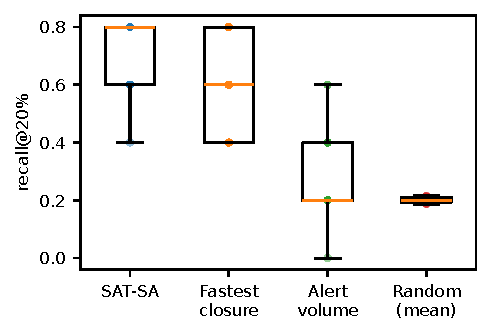
\includegraphics[width=0.5\linewidth]{figures/fig-prioritization.pdf}
\caption{Recall@20\% of generator-labelled pathological entities across
20 generated populations (PR01). The generator injects behaviours that
SAT-SA targets, so this is a controlled mechanism test, not an unbiased benchmark.}
\label{fig:prio}
\end{figure}

\subsection{One-worker ablation (RQ2)}
Removing one of the 16 workers at a time (Table~\ref{tab:ablation}),
fast-closure and negative-space carried recall on the catalog (0.600
and 0.600 without them; 1.000 with all workers).
Removing recurrence-without-remediation or coverage-gap \emph{raised} precision because
those workers emitted only undeclared families here. On five generated populations
(exploratory), mean recall@20\% was 0.760 with all workers and rose to
0.800 without the anomaly, recurrence, coverage-gap or
workflow-reconstruction worker, whereas removing the peer-benchmark or case-similarity
worker lowered it to 0.720. On these populations, therefore, some
workers add ranking noise to the measured metric.

We read this nuanced result narrowly. The full worker set spans a broader analytical
signal space than the generated populations exercise, and the ranking objective is
specific to the generator's pathological profile. The ablation therefore shows that
some workers can reduce this particular metric on these populations; worker utility
is task- and population-dependent (Section~\ref{sec:threats}).

\begin{table}[t]
\caption{One-worker ablation (A01): catalog micro precision/recall (5
scenarios, one database per scenario) and mean population recall@20\% (Pop.\ R@20; five seeds,
exploratory). Only workers whose removal changed a value are listed; ``--'' = unchanged from the full set.}
\label{tab:ablation}
\centering
\scriptsize
\begin{tabular}{@{}L{5.4cm}rrr@{}}
\toprule
Workers & Precision & Recall & Pop.\ R@20 \\
\midrule
All 16 & 0.556 & 1.000 & 0.760 \\
$-$ fast closure & 0.429 & 0.600 & 0.600 \\
$-$ negative space & 0.500 & 0.600 & 0.640 \\
$-$ evidence completeness & 0.500 & 0.800 & -- \\
$-$ recurrence without remediation & 0.714 & 1.000 & 0.800 \\
$-$ coverage gap & 0.625 & 1.000 & 0.800 \\
$-$ anomaly & -- & -- & 0.800 \\
$-$ workflow reconstruction & -- & -- & 0.800 \\
$-$ peer benchmark & -- & -- & 0.720 \\
$-$ case similarity & -- & -- & 0.720 \\
\bottomrule
\end{tabular}
\end{table}


\subsection{Imperfect evidence (RQ3)}
Each perturbed condition declared its family, affected records and expected validation
outcome before it ran, on a fresh tenant database. Validation matched the declared
contract in 245 of 245 conditions with an expectation
(Table~\ref{tab:robust}): malformed timestamps, chronology violations, missing columns
and duplicates with native identifiers were rejected. Two behaviours limit
interpretation (Fig.~\ref{fig:robust}). First, validation is all-or-nothing:
independent omission of records left dangling references and rejected the whole
submission in 3, 11 and
14 of 25 replicates at 10, 25 and 50\% omission, whereas
referentially consistent omission was never rejected and changed the emitted finding
families in 1, 11 and 15
replicates. Second, \emph{stale and contradictory evidence is accepted silently}: all
15 conditions with records outside the assessment period were
accepted without warning and without any change to findings or risk, and contradictory
dispositions or a closed case with an open alert produced no finding. SAT-SA
implements no period, recency or cross-record consistency validation.

\begin{table}[t]
\caption{Imperfect-evidence conditions by family (R01b). Rejected = whole submission
rejected by validation; changed = emitted finding families differed from the paired
control; ``--'' = no condition rejected (all analysed). Validation matched its declared contract in 245 of
245 conditions with an expectation.}
\label{tab:robust}
\centering
\scriptsize
\begin{tabular}{@{}lrrrr@{}}
\toprule
Family & Conditions & Rejected & Analysed & Findings changed \\
\midrule
Missingness & 173 & 33 & 140 & 43 \\
Duplication & 34 & 25 & 9 & 5 \\
Malformation & 15 & 15 & 0 & 0 \\
Conflict & 18 & 5 & 13 & 4 \\
Staleness (no expectation) & 15 & -- & 15 & 0 \\
Control & 5 & -- & 5 & 0 \\
\bottomrule
\end{tabular}
\end{table}


\begin{figure}[!htbp]
\centering
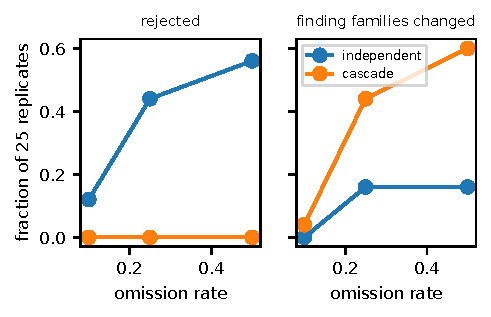
\includegraphics[width=0.55\linewidth]{figures/fig-robustness.pdf}
\caption{Record omission (R01b): independent omission is often rejected by
all-or-nothing validation; referentially consistent omission is accepted and changes
findings more often as the rate grows.}
\label{fig:robust}
\end{figure}

\subsection{Peer-cohort sensitivity (RQ4)}
Over 96 engineered cells (Fig.~\ref{fig:peer}), cohorts of two peers never
produced a finding, as Eq.~\eqref{eq:peer} requires three. With a tight cohort spread,
7 of eight subject values were flagged from three peers upward---every
value except the one at the cohort median. With a wide spread only extreme slow
subjects were flagged at small cohorts (2 at three peers), and fast
subjects only from five peers upward as the MAD narrowed (4 at five
peers). The peer rule is therefore sensitive to cohort size and dispersion: small or
heterogeneous cohorts miss deviations, and tight cohorts flag small ones.

\begin{figure}[!htbp]
\centering
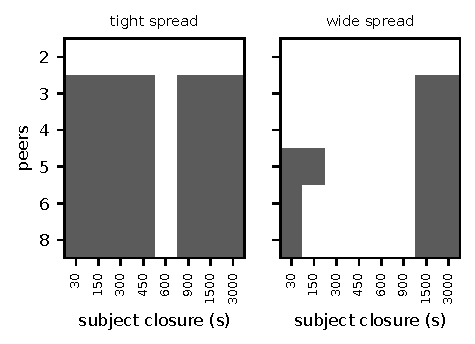
\includegraphics[width=0.68\linewidth]{figures/fig-peer.pdf}
\caption{Peer findings by cohort size, spread and subject closure value; dark cells
emitted a finding (P01, 96 cells).}
\label{fig:peer}
\end{figure}

\subsection{Orchestration cost and recovery (RQ5)}
On one machine with SQLite, 30 paired trials per mode gave median processing
times, excluding the human decision, of 1.276\,s (direct),
1.433\,s (LangGraph) and 0.976\,s (unreviewed benchmark
mode) (Table~\ref{tab:orch}). LangGraph minus direct was a median 0.096\,s
per workflow (95\% bootstrap \ensuremath{-}0.020 to 0.211\,s; the
interval includes zero), with 38 more database statements and
7 checkpoints per run; findings and risk were identical across modes
in every trial. Review with finalization added a median 0.318\,s over
unreviewed processing; finalization took 0.288\,s and receipt
verification 0.062\,s. Interruptions were injected at 6
points in both modes with 3 trials per cell: transient failures and
simulated crashes during analysis, before recommendations, at a worker restart during
review, and during finalization. \emph{In the evaluated interruption scenarios},
36 of 36 runs recovered, 36 with outputs
identical to the uninterrupted reference; completed stages were repeated
0 times, and every run had exactly one decision, one finalization and a
verifying receipt. Real process kills, network partitions and database failover were
not exercised.

\begin{table}[!htbp]
\caption{Orchestration cost on one machine with SQLite (O01, 30 paired
trials per mode; the human decision excluded). Median and p95 in seconds; Outside =
seconds outside the domain stages; DB = database statements. Graph $-$ direct: median
0.096\,s, 95\% bootstrap \ensuremath{-}0.020 to 0.211\,s
(graph slower in 19 of 30 pairs). Finalization took
0.288\,s, receipt verification 0.062\,s and run and
finding attestation 0.853\,s (medians).}
\label{tab:orch}
\centering
\small
\setlength{\tabcolsep}{4pt}
\begin{tabular}{@{}L{4.2cm}rrrr@{}}
\toprule
Mode & Median & p95 & Outside & DB \\
\midrule
Direct (reviewed) & 1.276 & 2.010 & 0.055 & 420 \\
LangGraph (reviewed) & 1.433 & 2.206 & 0.115 & 458 \\
Unreviewed benchmark mode & 0.976 & 1.655 & 0.029 & 253 \\
\bottomrule
\end{tabular}
\end{table}


\subsection{Integrity of the decided record (RQ6)}
On one finalized controlled workflow, each of 14 mutations was applied,
verified, restored and re-verified (Table~\ref{tab:trust}). Verification detected
13 of 13 mutations of signed state---decision action and
reason, finding, risk, recommendation, observation scope, source provenance,
submission record payload, artifact digest, canonical payload, receipt signature,
receipt public key and ledger chain---while the negative control (1
mutation of an unsigned operational queue field) still verified, as designed. These
results cover the tested mutation classes on one workflow; verification detects
alteration after the fact rather than preventing it (Section~\ref{sec:system}).

\begin{table}[!htbp]
\caption{Integrity mutation matrix on one finalized workflow (T01): 13
of 13 mutations of signed state detected; the unsigned control still
verified. Full targets are in the supplementary material.}
\label{tab:trust}
\centering
\small
\setlength{\tabcolsep}{4pt}
\begin{tabular}{@{}L{7.4cm}ll@{}}
\toprule
Mutated element & Expected & Observed \\
\midrule
Decision action; decision reason & tampered & tampered \\
Finding rationale; observation scope & tampered & tampered \\
Risk profile; recommendation & tampered & tampered \\
Source provenance; submission record payload & tampered & tampered \\
Artifact digest; canonical payload & tampered & tampered \\
Receipt signature; receipt public key & tampered & tampered \\
Ledger chain (predecessor hash) & tampered & tampered \\
Unsigned queue field (control) & verified & verified \\
\bottomrule
\end{tabular}
\end{table}


\section{External Evaluation and Failure Analysis}
\label{sec:external}

\paragraph{Setup.} The unchanged pipeline analysed the UCI-498 incident
log~\cite{amaral2018uci498}, a real ServiceNow event log of one organization's IT
service desk, with each final assignment group of sufficient size treated as an
entity: 50 groups, 22,604 of 24,918
incidents, 47,420 investigation-step proxies derived from work-state events
and 19,656 escalation proxies derived from reassignments. The only outcome
available is the final SLA flag. SLA labels were loaded only after SAT-SA's ranking
existed and never entered a submission. \emph{This is IT incident data, not SOC data};
it is, however, the log on which prior work demonstrated incident-management
compliance assessment~\cite{palma2024eurova} and modelled SLA
attainment~\cite{swain2022sla}.

\paragraph{Feasibility.} All 134,888 submitted rows were accepted
(0 rejected) and every group's analysis completed, with a median
of 9\,s per group.

\paragraph{Negative result.} SAT-SA's risk $R_e$ was not associated with the SLA-miss
rate: Spearman $\rho=\ensuremath{-}0.11$, 95\% bootstrap \ensuremath{-}0.42 to
0.21 (Table~\ref{tab:external}, Fig.~\ref{fig:external}). Slowest median
resolution reached $\rho=0.94$ (0.86 to
0.97), as expected for a timeliness outcome; reassignment rate
reached 0.37. Among the 12 groups in the top SLA-miss
quartile, SAT-SA's precision@10\% was 0.40 (random 0.25,
slowest resolution 1.00), and it needed to review 50
groups to find all of them (slowest resolution 24).

\begin{table}[t]
\caption{UCI-498 IT incident log (X02b, X03): Spearman association of group scores
with the SLA-miss rate over 50 assignment groups of one organization
(95\% seeded bootstrap intervals). Not SOC data.}
\label{tab:external}
\centering
\scriptsize
\begin{tabular}{@{}L{6.2cm}rr@{}}
\toprule
Group score & Spearman $\rho$ & 95\% interval \\
\midrule
SAT-SA risk $R_e$ & \ensuremath{-}0.11 & \ensuremath{-}0.42 to 0.21 \\
Incident volume & \ensuremath{-}0.15 & \ensuremath{-}0.42 to 0.16 \\
Reassignment rate & 0.37 & 0.08 to 0.60 \\
Slowest median resolution (upper reference) & 0.94 & 0.86 to 0.97 \\
\midrule
Execution-gap dimension of $R_e$ (X03) & \ensuremath{-}0.41 & \ensuremath{-}0.66 to \ensuremath{-}0.11 \\
Fast-closure prevalence (X03) & \ensuremath{-}0.70 & \ensuremath{-}0.82 to \ensuremath{-}0.52 \\
\bottomrule
\end{tabular}
\end{table}


\begin{figure}[t]
\centering
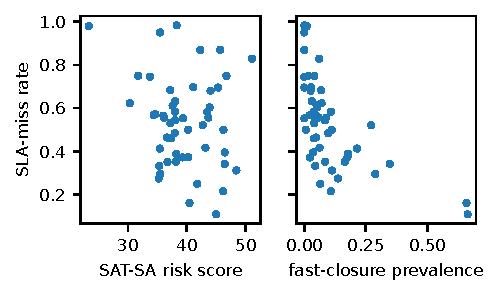
\includegraphics[width=0.78\linewidth]{figures/fig-external.pdf}
\caption{UCI-498 IT incident log (not SOC data): SAT-SA risk (left) and fast-closure
prevalence (right) against the SLA-miss rate; one point per assignment group
(50 groups; X02b, X03).}
\label{fig:external}
\end{figure}

\paragraph{Failure analysis.} A diagnostic analysis (X03) on the same data changed no
detector, threshold or weight. It attributes the result to four causes.
\emph{(i) Construct mismatch (primary).} On a service desk, fast resolution is the
goal: the prevalence of fast closures was \emph{negatively} associated with SLA misses
($\rho=\ensuremath{-}0.70$, \ensuremath{-}0.82 to \ensuremath{-}0.52). SAT-SA treats
fast closure of a security alert as possible skipped investigation, so its execution-gap
dimension, which this signal drives, ran opposite to the outcome
($\rho=\ensuremath{-}0.41$, \ensuremath{-}0.66 to \ensuremath{-}0.11). SLA
timeliness and supervisory execution quality are different constructs, and here they
move in opposite directions. \emph{(ii) Detector saturation.} 4 detector
families fired for every group although their input conditions varied widely---cases
without any step 1.7\% to 78.4\% of cases, medium-or-higher alerts
with fewer than two steps 5.2\% to 85.9\%. Existence rules
cannot discriminate submissions with thousands of tickets, and Eq.~\eqref{eq:risk}
adds near-constant amounts for them because it ignores prevalence; risk still took
49 distinct values and was unrelated to volume
($\rho=0.02$). \emph{(iii) Missing supervisory dimensions.}
3 of the 7 risk dimensions had no input data;
investigation steps and escalations are proxies (state changes and reassignments), and
monitoring coverage is unavailable. \emph{(iv) A minor adapter artifact.} The log has
no step notes; the adapter submits empty notes, which satisfy a repeated-investigation
rule in 39 groups. The analysis found no temporal or label defect: only
3 of 7,907 SLA misses occurred while another group held the
ticket, and reassigned incidents missed more often (53.8\% versus
21.5\%), consistent with the positive reassignment association.

\paragraph{Decision.} No risk-model change was made. Changing detectors or weights to
raise the correlation with SLA misses would optimize SAT-SA toward a timeliness
construct it does not claim to measure, using the evaluation data for tuning. We
therefore read X02b and X03 as \emph{feasibility and construct-validity evidence}, not
as external validation of effectiveness: on data whose outcome measures a different
construct and that lacks investigation, escalation and coverage semantics, SAT-SA's
supervisory signals did not transfer.

\section{Discussion}
\label{sec:discussion}

\paragraph{Multi-signal supervision versus simple heuristics.} The controlled results
show the mechanisms working as specified, but they do not show that the multi-worker
design adds value over transparent rules: fixed-threshold and MAD rules tie the
fast-closure detector, a fastest-median-closure ranking equals or nearly equals SAT-SA
in most generated populations---populations that favour SAT-SA by construction---and
four workers \emph{lowered} population recall in the ablation. This is consistent with
a generator whose pathological profile includes fast closures; more elaborate workers
can only earn their place on data where pathologies are not separable by one rate, and
the evidence here neither establishes nor rules out that they do. For a supervisor, a small set of transparent
rates may be a reasonable first instrument, with record-cited findings serving as the
explanation layer rather than the ranking signal.

\paragraph{Mechanism validation versus external validity.} Controlled experiments with
construction labels answer whether each mechanism does what it declares; they cannot
answer whether its output reflects supervisory quality. The external evaluation shows
why the distinction matters: the same fast-closure signal that is a warning in a SOC is
a success indicator in a service desk, so a construct defined for one setting inverts
in the other. The methodological lesson generalizes beyond SAT-SA: an external outcome
used to ``validate'' a supervisory score must measure the same construct, and a
negative association with a different construct is evidence about constructs, not a
defect to tune away. The external study also exposed a design limitation within SAT-SA's
own domain---existence rules fused by summed confidence saturate on large
submissions---which calls for prevalence-aware scoring developed on held-out SOC data.

\paragraph{Orchestration versus overhead.} On this workload, checkpointed orchestration
cost a median 0.096\,s per workflow with an interval that includes zero, at
the price of 38 additional database statements; in exchange, all evaluated
interruptions recovered without duplicated decisions. Whether this trade holds under
load, on PostgreSQL or across machines was not measured.

\paragraph{Integrity versus cost.} Finalization and verification are sub-second on this
machine, and the tested alterations of the decided record were detected. The guarantee
is narrow by construction: it binds what was analysed and decided, and it is only as
strong as key custody, which was not evaluated.

\paragraph{Peer analysis versus cohort dependence.} Peer comparison is the most
supervisor-specific signal, but P01 shows that its output is a function of cohort size
and spread as much as of the subject. Cohort definition is therefore a supervisory
decision that should be recorded and reviewed with the finding.

\paragraph{The human in the loop.} SAT-SA is decision support. Automation bias is a
documented risk for such tools~\cite{parasuraman2010automation,tilbury2024automationbias};
without a study with supervisors we cannot say whether record-cited findings help or
anchor their judgement.

\section{Threats to Validity and Limitations}
\label{sec:threats}

\paragraph{Construct validity.} Controlled labels are construction labels written by
the system's developers. The external outcome (SLA miss) measures timeliness, not
supervisory execution quality, and investigation and escalation are proxies there.
Risk scores have no validated meaning as probabilities or severities.

\paragraph{Internal validity.} Populations for prioritization and ablation come from
SAT-SA's own generator, which injects the behaviours its detectors target and favours
SAT-SA; the ranking results are therefore controlled mechanism evidence, not an
unbiased benchmark. Precision depends on database layout. Thresholds and confidence
rules were set by design, never fitted, and never tuned on independent development
data.

\paragraph{Worker complexity.} The one-worker ablation does not show that all
16 analytical workers are necessary or that the set is optimal: on the
generated populations, removing some workers raised the ranking metric. Whether any
worker helps or harms on real supervisory data is untested.

\paragraph{External validity.} The evaluation is predominantly synthetic and
controlled. There is no SOC data from a real organization; the external dataset is one
IT service desk; generated populations have 20 entities, which makes
top-$k$ estimates coarse; the ablation population analysis uses five seeds.

\paragraph{Statistical conclusion validity.} Intervals are descriptive, seeded and
uncorrected across many comparisons; no hypothesis is tested. Timing results are
repeated runs on one machine and do not generalize across hardware, databases or load.
Recovery was tested with injected exceptions at worker boundaries, not real process
kills, partitions or database failover.

\paragraph{Human factors.} A human-evaluation protocol exists but \emph{no study was
executed}: there are no participants and no usability or decision-quality results. An
expert-label pipeline exists but \emph{no expert-labelled data exist}.

\paragraph{Systems and deployment validity.} All measurements used SQLite and local
storage on one machine. The local API and worker processes passed 18 HTTP
smoke checks (0 failed). Docker was not available, so the container image
and compose topology were not executed; SeaweedFS object storage, the CI topology job
and any hosted deployment were not executed. PostgreSQL played no part in any reported
measurement. (After the evidence freeze, the schema migrations and the database test
suite were run against a local PostgreSQL instance during maintenance; this is not
part of the evaluation.) The results therefore characterize the evaluated
configuration, not the production deployment architecture.

\section{Reproducibility and Artifact Availability}
\label{sec:repro}

\paragraph{Evidence chain.} Each reported number is generated from a canonical bundle
in a hash-verified evidence freeze; the build verifies bundle hashes before reading
them, and an audit regenerates all paper values, tables and figures and compares them
byte for byte, rejects hand-typed decimals and checks every citation against a
verified literature matrix.

\paragraph{Reproduction levels.} We claim only what was demonstrated.
\emph{Level~1, artifact verification (demonstrated):} every recorded hash is recomputed,
in the working repository and in fresh clones; edited manifests, raw results, metrics
and configurations are rejected. \emph{Level~2, result regeneration (demonstrated):}
paper values, tables and figures regenerate byte-identically from the frozen bundles.
\emph{Level~3, experiment reproduction (demonstrated for two experiments):} re-running
the integrity mutation matrix (T01) and the peer sweep (P01) under new experiment
identifiers reproduced their analytical outputs; timing experiments reproduce only in
distribution. \emph{Level~4, environment reproduction (not demonstrated):} a container
image and compose topology exist but were not executed; all runs used one Windows
machine. \emph{Level~5, external-data reproduction (demonstrated once, same machine):}
the external experiment was executed twice from the checksum-verified public dataset
with identical analytical outputs; there is no third-party reproduction.

\paragraph{Code and data availability.} The source code, experiment runners, evidence
freeze, paper data layer and literature-search scripts are public under the MIT licence
at \url{https://github.com/PrathamKapoor/SAT-SA-with-PQC}. The reported evaluation is
identified by commits, not by a branch: each experiment was executed from the source
commit recorded in its bundle manifest (listed in the supplementary material), and the
frozen evidence set \texttt{satsa-evidence-freeze-v2} (canonical code commit
\texttt{837d1ef}) was committed as \texttt{85b7763}. All controlled data
are synthetic and regenerate from the recorded seeds and configurations. The external
dataset~\cite{amaral2018uci498} is public under a Creative Commons Attribution (CC BY) licence and is not
redistributed; the
experiment downloads it and verifies its checksum. No personal data, no data from a
real SOC and no human-participant data were used.

\section{Conclusion}
\label{sec:conclusion}

We evaluated record-level supervisory analytics for SOCs as implemented in SAT-SA:
rule-based analysis of the records a monitored organization submits, saturating risk
fusion and ranking, a human supervisory decision, and cryptographic binding of that
decision to the analysed state. Under controlled conditions the mechanisms behave as
specified---declared findings are emitted, validation follows its contract, the tested
alterations of the decided record are detected, and the evaluated interruptions
recover---but simple rules match much of the detection and ranking performance even on
generated populations that favour SAT-SA by construction, not every analytical worker
improved the ranking metric, and stale and contradictory evidence passes silently. On a public IT incident log the
supervisory risk did not track the only outcome available, because that outcome
measures timeliness, which the fast-closure signal treats in the opposite direction,
and because existence rules saturate at scale. What can be concluded is therefore
mechanism-level: the pipeline is inspectable and behaves as designed, while its
usefulness for supervision is untested. The evidence needed next is not more
controlled experiments but SOC records with independent outcomes held out from
development, expert-labelled findings, a study with supervisors, prevalence-aware
scoring and consistency checks for stale and conflicting records, and validation of
the containerized PostgreSQL deployment.

\begin{credits}
\subsubsection{Ethics approval.}
This study did not involve human participants, human-subject research, or
identifiable personal data; therefore, ethics approval was not required.
\end{credits}


\bibliographystyle{splncs04}
\bibliography{references}

\end{document}
